\documentclass[a4paper]{report}
\usepackage[utf8]{inputenc}
\usepackage[portuguese]{babel}
\usepackage{hyperref}
\usepackage{a4wide}
\hypersetup{pdftitle={VC - Turorial 1},
pdfauthor={José Ferreira, Luís Pereira},
colorlinks=true,
urlcolor=blue,
linkcolor=black}
\usepackage{subcaption}
\usepackage{listings}
\usepackage{booktabs}
\usepackage{multirow}
\usepackage{appendix}
\usepackage{tikz}
\usepackage{authblk}
\usepackage{bashful}
\usepackage{verbatim}
\usepackage{amssymb}
\usepackage{multirow}
\usepackage{mwe}
\usepackage{float}
\usetikzlibrary{positioning,automata,decorations.markings}

\begin{document}

\title{VC - Turorial 1}
\author{José Ferreira (A83683), Luís Pereira (A86265)}
\date{\today}

\begin{center}
    \begin{minipage}{0.75\linewidth}
        \centering
        
\includegraphics[width=0.4\textwidth]{images/eng.jpeg}\par\vspace{1cm}
        \vspace{1.5cm}
        \href{https://www.uminho.pt/PT}
        {\color{black}{\scshape\LARGE Universidade do Minho}} \par
        \vspace{1cm}
        \href{https://www.di.uminho.pt/}
        {\color{black}{\scshape\Large Departamento de Informática}} \par
        \vspace{1.5cm}
        \maketitle
    \end{minipage}
\end{center}

\tableofcontents

\pagebreak
\chapter{Introdução}
No âmbito da unidade curricular de Visão por Computador, foi-nos proposto implementar dois tipos de programas.
Um deste programas tem como objetivo suavizar imagens. O outro outro tem a finalidade de detetar as bordas de uma imagem.
O objetivo deste projeto consiste em colocar à prova os nossos conhecimentos da linguagem \texttt{MATLAB} e a aplicação da teoria leccionada nas aulas da UC.

Ao longo deste relatório iremos descrever os algoritmos implementados para cada um dos programas assim como relatar as
diversas conclusões que obtivemos com os \textit{outputs} dos programas criados.

Primeiro descrevemos como forma implementados dois geradores de ruído, salt-n-pepper e gaussiano. Estes algoritmos foram criados com o objetivo de testar os vários algoritmos que foram desenvolvidos.

Em seguida apresentamos os algoritmos de smoothing implementados apresentando várias
comparações entre algoritmos de suavização implementados para os vários tipos de ruído criados.

Finalmente descrevemos como foi implementado um detetor de bordas. Para tal foi necessário a
implementação de vários algoritmos para chegar ao resultado final, sendo estes Gaussian Smoothing, Gradient Calculation,
Non-Maximum Supression, Double Threshold e Hysteresis Threshold. No final do capítulo é ainda comparado com outros
métodos usando uma função do \texttt{MATLAB} de nome \texttt{edge}.

\chapter{Noise}
Para introduzir ruído numa imagem foi criado uma função denominada de ruído.
Esta recebe uma matriz que representa uma imagem, o tipo de ruído a ser
utilizado e os parâmetros para esse ruído.

O ruído gaussiano consiste em calcular uma matriz de valores aleatórios e adicionar essa matriz a
matriz que representa a imagem. No caso deste ruído o parâmetro passado representa a variância
dos valores calculados. Caso o ruído seja \textit{salt-n-peppper} pixeis aleatórios na imagem são 
convertidos para branco ou para preto, neste caso o parâmetro representa a percentagem de
ocorrência dos pixeis.

\begin{figure}[H]
\centering
\begin{minipage}{.3\textwidth}
  \centering
    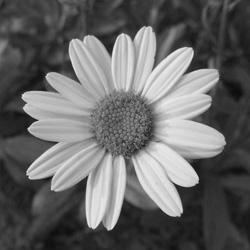
\includegraphics[width=0.95\textwidth]{images/Smooth/flower.jpg}
    \captionof{figure}{Original}
\end{minipage}%
\begin{minipage}{.3\textwidth}
  \centering
    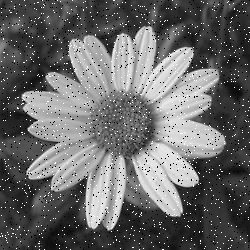
\includegraphics[width=0.95\textwidth]{images/Smooth/flower_salt-n-pepper_0.05.png}
    \captionof{figure}{Salt-n-pepper}
\end{minipage}%
\begin{minipage}{.3\textwidth}
  \centering
  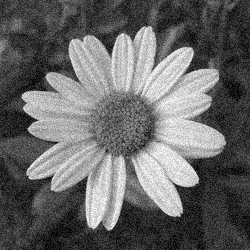
\includegraphics[width=0.95\textwidth]{images/Smooth/flower_gaussian_0.1.png}
  \captionof{figure}{Gaussian}
\end{minipage}
\end{figure}

\chapter{Smooth Images}
\section{Spatial Smoothing para Ruído Salt-n-pepper}
Ao longo desta secção iremos comparar os diversos tipos de smoothing espaciais implementados aplicando-os sobre o ruído
salt-n-pepper descrito anteriormente.

Comparação entre diferentes tamanhos de kernel para smoothing espacial usando média. Como se pode observar, quanto maior o tamanho do kernel mais desfocada fica a imagem.
\begin{figure}[H]
\centering
\begin{minipage}{.3\textwidth}
  \centering
    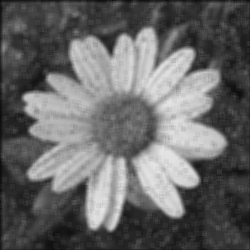
\includegraphics[width=0.95\textwidth]{images/Smooth/spatial-salt-n-pepper/flower_smooth_spatial_average_5_0.8.png}
    \captionof{figure}{size: 5}
\end{minipage}%
\begin{minipage}{.3\textwidth}
  \centering
    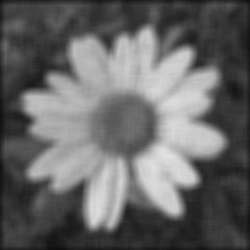
\includegraphics[width=0.95\textwidth]{images/Smooth/spatial-salt-n-pepper/flower_smooth_spatial_average_10_0.8.png}
    \captionof{figure}{size: 10}
\end{minipage}%
\begin{minipage}{.3\textwidth}
  \centering
  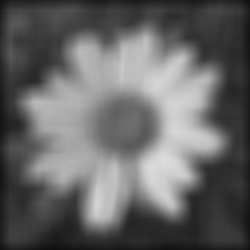
\includegraphics[width=0.95\textwidth]{images/Smooth/spatial-salt-n-pepper/flower_smooth_spatial_average_20_0.8.png}
  \captionof{figure}{size: 20}
\end{minipage}
\end{figure}

Comparação entre diferentes tamanhos de kernel para smoothing com gauss. Neste caso, a diferença entre diversos tamanho
de kernel torna-se inexistente. Tal deve-se ao facto de à medida que o tamanho do kernel aumenta os pixeis mais afastados
tem um peso cada vez menor e por isso menor influencia sobre o pixel a ser tratado.

\begin{figure}[H]
\centering
\begin{minipage}{.3\textwidth}
  \centering
    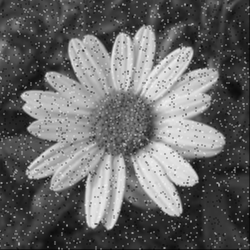
\includegraphics[width=0.95\textwidth]{images/Smooth/spatial-salt-n-pepper/flower_smooth_spatial_gaussian_5_2.png}
    \captionof{figure}{size: 5}
\end{minipage}%
\begin{minipage}{.3\textwidth}
  \centering
    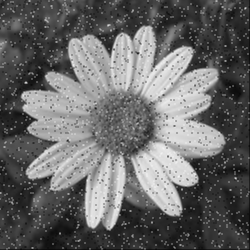
\includegraphics[width=0.95\textwidth]{images/Smooth/spatial-salt-n-pepper/flower_smooth_spatial_gaussian_10_2.png}
    \captionof{figure}{size: 10}
\end{minipage}%
\begin{minipage}{.3\textwidth}
  \centering
  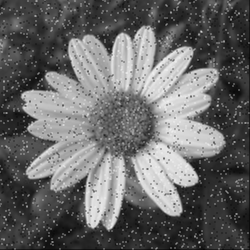
\includegraphics[width=0.95\textwidth]{images/Smooth/spatial-salt-n-pepper/flower_smooth_spatial_gaussian_20_2.png}
  \captionof{figure}{size: 20}
\end{minipage}
\end{figure}

Comparação entre diferentes tamanhos de kernel para smoothing com mediana. Neste caso, quanto maior o tamanho do kernel
mais detalhe se perde sendo que quando nos aproximamos do valor 20 a forma da imagem original fica irreconhecível. No
entanto, No tamanho 5 do kernel todo o ruído salt-n-pepper desaparece.

\begin{figure}[H]
\centering
\begin{minipage}{.3\textwidth}
  \centering
    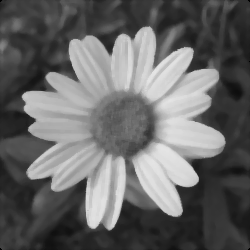
\includegraphics[width=0.95\textwidth]{images/Smooth/spatial-salt-n-pepper/flower_smooth_spatial_median_5_1.png}
    \captionof{figure}{size: 5}
\end{minipage}%
\begin{minipage}{.3\textwidth}
  \centering
    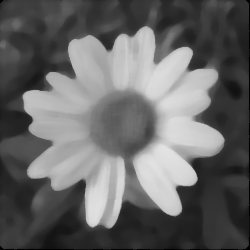
\includegraphics[width=0.95\textwidth]{images/Smooth/spatial-salt-n-pepper/flower_smooth_spatial_median_10_1.png}
    \captionof{figure}{size: 10}
\end{minipage}%
\begin{minipage}{.3\textwidth}
  \centering
  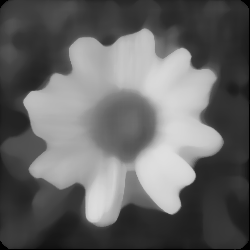
\includegraphics[width=0.95\textwidth]{images/Smooth/spatial-salt-n-pepper/flower_smooth_spatial_median_20_1.png}
  \captionof{figure}{size: 20}
\end{minipage}
\end{figure}

Assim, com base nas imagens acima apresentadas, o melhor tipo de smoothing para o ruído salt-n-pepper é o que utiliza 
a mediana.

\section{Spatial Smoothing para Ruído Gaussiano}
Ao longo desta secção iremos comparar os diversos tipos de smoothing espaciais implementados aplicando-os sobre o ruído
gaussiano descrito anteriormente.

Comparação entre diferentes tamanhos de kernel para smoothing espacial usando media. Neste caso quanto maior o
tamanho do kernel mais desfocado fica a imagem original.
\begin{figure}[H]
\centering
\begin{minipage}{.3\textwidth}
  \centering
    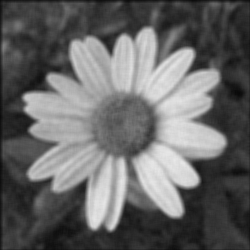
\includegraphics[width=0.95\textwidth]{images/Smooth/spatial-gaussian/flower_smooth_spatial_average_5_0.8.png}
    \captionof{figure}{size: 5}
\end{minipage}%
\begin{minipage}{.3\textwidth}
  \centering
    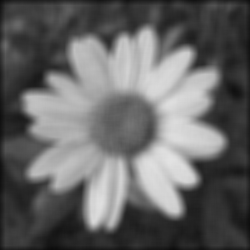
\includegraphics[width=0.95\textwidth]{images/Smooth/spatial-gaussian/flower_smooth_spatial_average_10_0.8.png}
    \captionof{figure}{size: 10}
\end{minipage}%
\begin{minipage}{.3\textwidth}
  \centering
  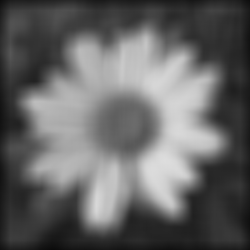
\includegraphics[width=0.95\textwidth]{images/Smooth/spatial-gaussian/flower_smooth_spatial_average_20_0.8.png}
  \captionof{figure}{size: 20}
\end{minipage}
\end{figure}

Comparação entre diferentes tamanhos de kernel para smoothing espacial usando gaussian. Neste caso a alteração do
tamanho do kernel não modifica muito o resultado final.
\begin{figure}[H]
\centering
\begin{minipage}{.3\textwidth}
  \centering
    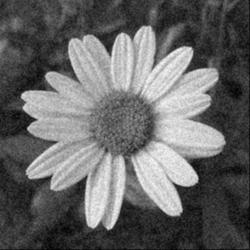
\includegraphics[width=0.95\textwidth]{images/Smooth/spatial-gaussian/flower_smooth_spatial_gaussian_5_2.png}
    \captionof{figure}{size: 5}
\end{minipage}%
\begin{minipage}{.3\textwidth}
  \centering
    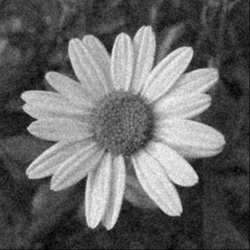
\includegraphics[width=0.95\textwidth]{images/Smooth/spatial-gaussian/flower_smooth_spatial_gaussian_10_2.png}
    \captionof{figure}{size: 10}
\end{minipage}%
\begin{minipage}{.3\textwidth}
  \centering
  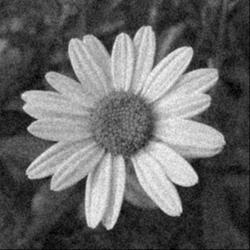
\includegraphics[width=0.95\textwidth]{images/Smooth/spatial-gaussian/flower_smooth_spatial_gaussian_20_2.png}
  \captionof{figure}{size: 20}
\end{minipage}
\end{figure}

Comparação entre diferentes tamanhos de kernel para smoothing espacial usando mediana. Neste caso a imagem
fica muito desfocada e quanto maior o tamanho do kernel mais detalhes se perdem.
\begin{figure}[H]
\centering
\begin{minipage}{.3\textwidth}
  \centering
    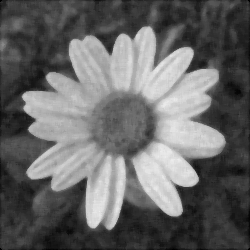
\includegraphics[width=0.95\textwidth]{images/Smooth/spatial-gaussian/flower_smooth_spatial_median_5_1.png}
    \captionof{figure}{size: 5}
\end{minipage}%
\begin{minipage}{.3\textwidth}
  \centering
    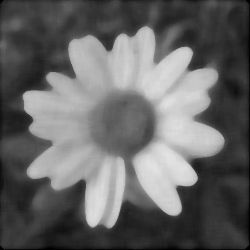
\includegraphics[width=0.95\textwidth]{images/Smooth/spatial-gaussian/flower_smooth_spatial_median_10_1.png}
    \captionof{figure}{size: 10}
\end{minipage}%
\begin{minipage}{.3\textwidth}
  \centering
  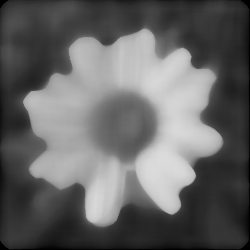
\includegraphics[width=0.95\textwidth]{images/Smooth/spatial-gaussian/flower_smooth_spatial_median_20_1.png}
  \captionof{figure}{size: 20}
\end{minipage}
\end{figure}

Observando os resultados acima, o tipo de smoothing que reduz mais ruído sem perder detalhe acaba por ser
o smoothing gaussiano.

\section{Frequency Smoothing para Ruído Salt-n-pepper}
Ao longo desta secção iremos comparar os diversos tipos de smoothing em frequência implementados aplicando-os sobre o ruído
salt-n-pepper descrito anteriormente.

Comparação entre diferentes sigmas para smoothing por frequência usando gauss. Neste caso quanto maior o sigma melhor o resultado final da imagem.
\begin{figure}[H]
\centering
\begin{minipage}{.3\textwidth}
  \centering
    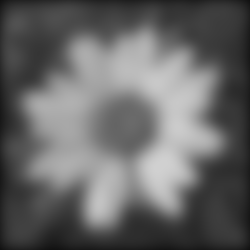
\includegraphics[width=0.95\textwidth]{images/Smooth/frequency-salt-n-pepper/flower_smooth_frequency_gaussian_10_1.png}
    \captionof{figure}{sigma: 10}
\end{minipage}%
\begin{minipage}{.3\textwidth}
  \centering
    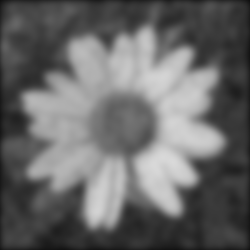
\includegraphics[width=0.95\textwidth]{images/Smooth/frequency-salt-n-pepper/flower_smooth_frequency_gaussian_20_1.png}
    \captionof{figure}{sigma: 20}
\end{minipage}%
\begin{minipage}{.3\textwidth}
  \centering
  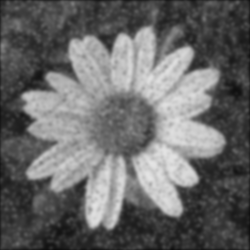
\includegraphics[width=0.95\textwidth]{images/Smooth/frequency-salt-n-pepper/flower_smooth_frequency_gaussian_50_1.png}
  \captionof{figure}{sigma: 50}
\end{minipage}
\end{figure}

Comparação entre diferentes cutoffs (com ordem fixa de 2) para smoothing por frequência usando Butterworth. Neste caso quanto maior o cutoff melhor a qualidade da imagem.
\begin{figure}[H]
\centering
\begin{minipage}{.3\textwidth}
  \centering
    
\includegraphics[width=0.9\textwidth]{images/Smooth/frequency-salt-n-pepper/flower_smooth_frequency_Butterworth_2_5.png}
    \captionof{figure}{cutoff: 5}
\end{minipage}%
\begin{minipage}{.3\textwidth}
  \centering
    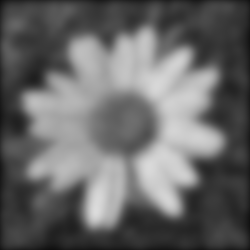
\includegraphics[width=0.9\textwidth]{images/Smooth/frequency-salt-n-pepper/flower_smooth_frequency_Butterworth_2_20.png}
    \captionof{figure}{cutoff: 10}
\end{minipage}%
\begin{minipage}{.3\textwidth}
  \centering
  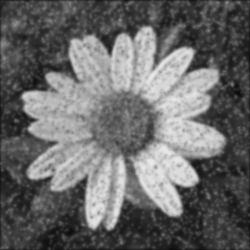
\includegraphics[width=0.9\textwidth]{images/Smooth/frequency-salt-n-pepper/flower_smooth_frequency_Butterworth_2_80.png}
  \captionof{figure}{cutoff: 20}
\end{minipage}
\end{figure}

Neste caso o melhor filtro por frequência  para o ruído gaussiano acaba por ser usando Butterworth.

\section{Frequency Smoothing para Ruído Gaussiano}
Ao longo desta secção iremos comparar os diversos tipos de smoothing em frequência implementados aplicando-os sobre o ruído
gaussiano descrito anteriormente.

Comparação entre diferentes sigmas para smoothing por frequência usando gauss.
\begin{figure}[H]
\centering
\begin{minipage}{.3\textwidth}
  \centering
    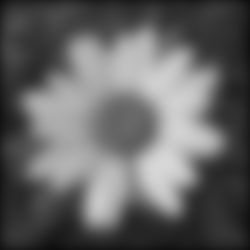
\includegraphics[width=0.9\textwidth]{images/Smooth/frequency-gaussian/flower_smooth_frequency_gaussian_10_1.png}
    \captionof{figure}{sigma: 10}
\end{minipage}%
\begin{minipage}{.3\textwidth}
  \centering
    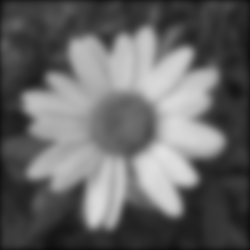
\includegraphics[width=0.9\textwidth]{images/Smooth/frequency-gaussian/flower_smooth_frequency_gaussian_20_1.png}
    \captionof{figure}{sigma: 20}
\end{minipage}%
\begin{minipage}{.3\textwidth}
  \centering
  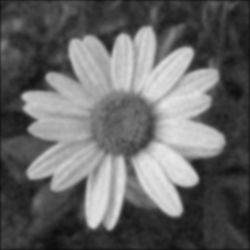
\includegraphics[width=0.9\textwidth]{images/Smooth/frequency-gaussian/flower_smooth_frequency_gaussian_50_1.png}
  \captionof{figure}{sigma: 50}
\end{minipage}
\end{figure}

Comparação entre diferentes cutoffs (com ordem fixa de 2) para smoothing por frequência usando Butterworth.
\begin{figure}[H]
\centering
\begin{minipage}{.3\textwidth}
  \centering
    
\includegraphics[width=0.9\textwidth]{images/Smooth/frequency-gaussian/flower_smooth_frequency_Butterworth_2_5.png}
    \captionof{figure}{cutoff: 5}
\end{minipage}%
\begin{minipage}{.3\textwidth}
  \centering
    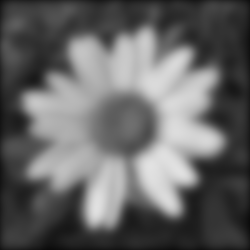
\includegraphics[width=0.9\textwidth]{images/Smooth/frequency-gaussian/flower_smooth_frequency_Butterworth_2_20.png}
    \captionof{figure}{cutoff: 10}
\end{minipage}%
\begin{minipage}{.3\textwidth}
  \centering
  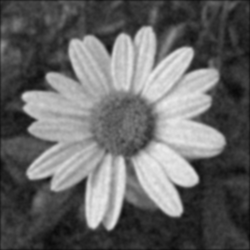
\includegraphics[width=0.9\textwidth]{images/Smooth/frequency-gaussian/flower_smooth_frequency_Butterworth_2_80.png}
  \captionof{figure}{cutoff: 20}
\end{minipage}
\end{figure}

Neste caso o melhor filtro por frequência  para o ruído gaussiano acaba por ser usando Gauss.

\chapter{Detect Edges}
\section{Canny Detector}
De modo a serem detetadas as bordas numa imagem foi implementado um detetor de
bordas, tendo por base um desenvolvido por John F. Canny em 1986. Este utiliza um algoritmo multi-estágios
com o objetivo de detetar várias bordas numa imagem.

John Canny também propôs como um detector de bordas deveria ser composto para ser
considerado ideal:
\begin{itemize}
    \item \textbf{Boa Detecção} - O algoritmo tem ser capaz de identificar todas as bordas possíveis numa imagem.
    \item \textbf{Boa Localização} - As bordas encontradas têm de se encontrar o mais próximo possível das bordas da imagem original.
    \item \textbf{Resposta Mínima} - Cada borda da imagem tem de ser marcada uma única vez. O ruído da imagem não pode criar falsas bordas.
\end{itemize}


Para a demonstração deste detetor foram escolhidos alguns \textit{inputs}. Um dos \textit{inputs} é uma imagem com ruído gaussiano. Naturalmente, para este valor foi escolhido um dos \textit{outputs} do capítulo anterior, já que neste foi necessário adicionar ruído gaussiano a uma dada imagem.

\begin{figure}[H]
    \centering
        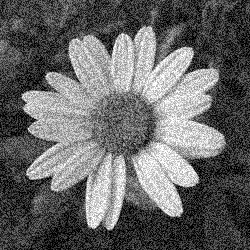
\includegraphics[width=0.3\textwidth]{images/Smooth/flower_gaussian_0.2.png}
        \caption{Imagem com ruído gaussiano}
\end{figure}

Foram também escolhidos um \textbf{sigma}, um \textbf{x} e um \textbf{y}, usados para suavizar a imagem com ruído gaussiano. Serão explicados como estes interagem com a imagem mais à frente.\\
 
Antes do início da execução do detetor é acrescentado uma moldura preta à imagem, de tamanho x no eixo do x e de y no eixo do y, para que os kernels possam ser executados em todos os pixeis. No entanto, é de notar que ao longo do algoritmo são criadas bordas falsas, que poderiam ser removidas com uma moldura superior, como o caso de uma moldura formada pelo estender da imagem com os pixeis que estão nas arestas da imagem.



\section{Gaussian Smoothing}
Como mencionado anteriormente, esta função necessita de todos os inputs dados a este programa. Com a pequena nuance da imagem já ir processada com a moldura. O objetivo desta função é suavizar a imagem tentando reduzir ao máximo o ruído, sem comprometer muito a qualidade da imagem. Com a imagem processada e os respectivos valores de sigma, x e y esta função cria o kernel gaussiano. O valor de sigma altera a potência deste filtro, quanto maior o seu valor mais a imagem fica suavizada, mas também fica com mais \textit{blur}. Como se demonstra nas imagens abaixo com valores de sigma iguais a 0.8 e 1.8.

\begin{figure}[H]
\centering
\begin{minipage}{.5\textwidth}
  \centering
    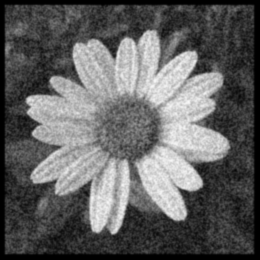
\includegraphics[width=0.9\textwidth]{images/Canny/flowerSigma0.8.png}
  \captionof{figure}{Imagem suavizada com sigma=0.8}
\end{minipage}%
\begin{minipage}{.5\textwidth}
  \centering
  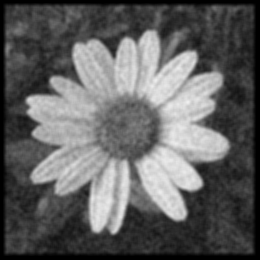
\includegraphics[width=0.9\textwidth]{images/Canny/flowerSigma1.8.png}
  \captionof{figure}{Imagem suavizada com sigma=1.8}
\end{minipage}
\end{figure}

Depois existem os valores de x e y, estes simbolizam o tamanho do kernel, ou seja, quantos pixeis vão contribuir para a suavização do pixel a ser processado, desta forma se x e y forem iguais a 3 (size=3), o número dos pixeis adjacentes ao pixel que vão contribuir para o seu processamento são (3*3)-1=8. Claramente, os pixeis mais longe do pixel a ser processado terão menor contribuição para o seu valor final, como é possível identificar na imagem seguinte.


\begin{figure}[H]
    \centering
        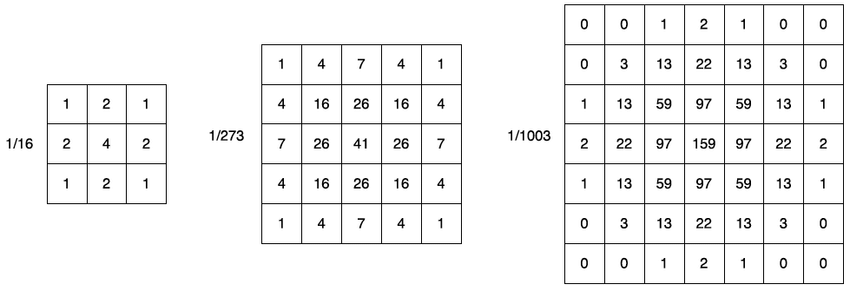
\includegraphics[width=0.9\textwidth]{images/Canny/GaussianFilters.png}
        \caption{Filtros Gaussianos de diferentes tamanhos}
\end{figure}


Quando aplicados estes kernels à imagem é possível obter as seguintes imagens para x e y iguais a 3 (size=3), e x e y iguais a 13 (size=13). 

\begin{figure}[H]
\centering
\begin{minipage}{.5\textwidth}
  \centering
    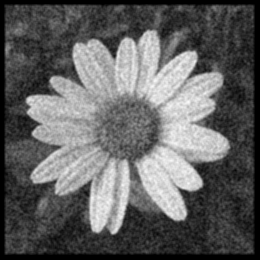
\includegraphics[width=0.9\textwidth]{images/Canny/flowerSize3.png}
  \captionof{figure}{Imagem suavizada com size=3}
\end{minipage}%
\begin{minipage}{.5\textwidth}
  \centering
  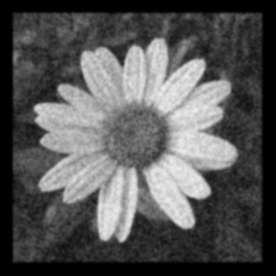
\includegraphics[width=0.9\textwidth]{images/Canny/flowerSize13.png}
  \captionof{figure}{Imagem suavizada com size=13}
\end{minipage}
\end{figure}

Consegue-se identificar que a moldura da imagem obtém tamanhos diferentes consoante o valor de x e y, aumentando quando estes também aumentam. Também se observa uma maior suavização quanto maior o kernel usado.


\section{Gradient}
De seguida a imagem processada na função anterior é enviada para a função Gradient. Como o nome
indica, esta função é responsável pela computação dos gradientes verticais e horizontais da imagem,
assim como as suas direções.\\

Este algoritmo tira proveito dos kernels de Sobel para realizar convoluções na imagem. É usado um
kernel para a convolução no eixo do x, assim como outra no eixo do y.

\begin{figure}[H]
    \centering
        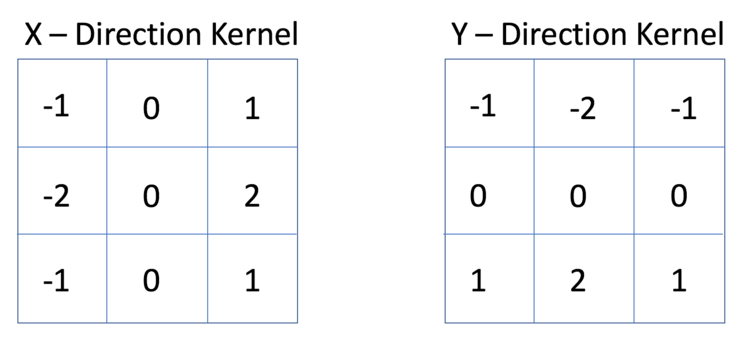
\includegraphics[width=0.6\textwidth]{images/Canny/SobelKernels.png}
        \caption{Filtros Gaussianos de diferentes tamanhos}
\end{figure}

 Mais uma vez cada elemento da matriz vai especificar a importância dos pixeis adjacentes, para a
 convolução no pixel a ser processado. São então calculadas as convoluções nos eixos do x e y,
 resultando nas duas seguintes imagens.


\begin{figure}[H]
\centering
\begin{minipage}{.5\textwidth}
  \centering
    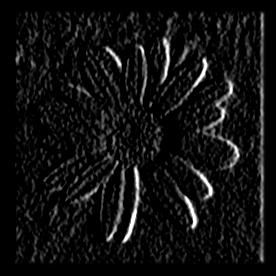
\includegraphics[width=0.9\textwidth]{images/Canny/flowerIx.png}
  \captionof{figure}{Gradiente da imagem no eixo do x}
\end{minipage}%
\begin{minipage}{.5\textwidth}
  \centering
  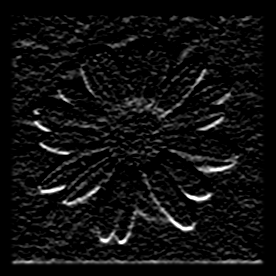
\includegraphics[width=0.9\textwidth]{images/Canny/flowerIy.png}
  \captionof{figure}{Gradiente da imagem no eixo do y}
\end{minipage}
\end{figure}

Através destas é calculado a imagem gradiente através da hipotenusa entre as duas e dividindo o
valor resultante pelo valor máximo dentre todos os pixeis que compõem a imagem resultante. É ainda
calculada a matriz com as direções através do arco tangente entre as mesmas duas convoluções, para
ser enviada à função seguinte.  


\begin{figure}[H]
\centering
\begin{minipage}{.5\textwidth}
  \centering
    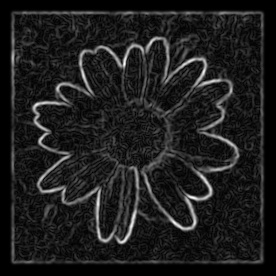
\includegraphics[width=0.9\textwidth]{images/Canny/flowerGrad.png}
  \captionof{figure}{Gradiente da imagem}
\end{minipage}%
\end{figure}


\section{NonMax}
Esta função vai receber os dois \textit{outputs} calculados pela função anterior, estes sendo a
imagem gradiente e as respetivas direções. Inicialmente, vai pegar na matriz de direções e
passa-las para os ângulos que estas representam, colocando-as numa nova matriz com esses valores.
De seguida vai passar por todos os pixeis da imagem gradiente e encontra quais os pixeis que têm o
valor máximo de intensidade na direção das bordas, utilizando a matriz calculada antes. Este
processo vai transformar as bordas iniciais, que podiam ter bordas densas, em bordas mais finas,
tendencialmente com apenas um pixel de espessura.\\

Como resultado desta função na imagem da flor, temos a seguinte imagem, onde realmente se consegue
observar uma elevada diminuição na espessura das bordas especialmente nas pétalas da flor.

\begin{figure}[H]
    \centering
        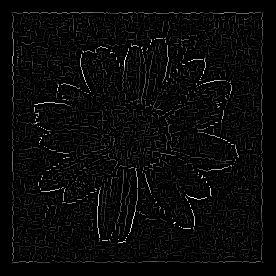
\includegraphics[width=0.38\textwidth]{images/Canny/flowerNonMax.png}
        \caption{Imagem após NonMax Supression}
\end{figure}


\section{Double Threshold}
O objetivo desta função é identificar 3 tipos de pixeis, podendo estes ser \textbf{fortes},
\textbf{fracos} ou \textbf{não relevantes}.

\begin{itemize}
    \item Pixeis \textbf{fortes} são pixeis que têm uma intensidade tão alta que se tem a certeza que vão fazer parte da borda final.
    \item Pixeis \textbf{fracos} são pixeis que têm uma intensidade que não é suficiente para ser considerados fortes, mas também não são tão fracos de modo a serem considerados não relevantes.
    \item Os pixeis \textbf{não relevantes} têm uma intensidade tão fraca que são retirados da imagem.
\end{itemize}

Para ser executado esta filtragem de pixeis é necessária a imagem calculada na função anterior, assim
como um rácio para cálculo do \textit{threshold} superior e outro para o \textit{threshold}
inferior. Através destes são calculados os verdadeiros \textit{thresholds}. São então percorridos
todos os pixeis da imagem comparando-os com os valores dos \textit{thresholds} calculados, criando
numa nova imagem com valores predefinidos, um valor para simbolizar pixel forte e outro para pixel
fraco, e os não relevantes colocados a preto. 

\begin{figure}[H]
    \centering
        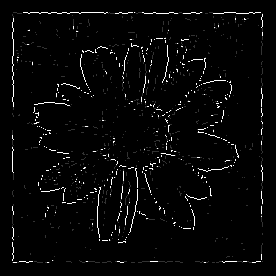
\includegraphics[width=0.38\textwidth]{images/Canny/flowerDoubleThreshold.png}
        \caption{Imagem após double threshold}
\end{figure}

Os \textit{thresholds} "ótimos" podem variar de imagem para imagem, de modo que se deve
experimentar com vários valores para se conseguir ter os resultados mais próximos do pretendido. Ao baixar muito os \textit{thresholds} começam a aparecer bordas a mais, ou então, ao subir os \textit{thresholds} começam a desaparecer bordas importantes para a imagem.


\section{Hysteresis Thresholding}
A função Hysteresis Thresholding tem por base o resultado dos thresholds calculados na função anterior. Consiste em transformar alguns dos pixeis fracos em pixeis fortes e outros em pixeis pretos. Ao percorrer a imagem, sempre que encontra um pixel fraco são percorridos os pixeis em volta deste e se algum destes for forte, este também se torna num pixel forte, caso contrário este fica preto.



\begin{figure}[H]
    \centering
        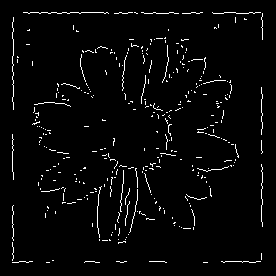
\includegraphics[width=0.4\textwidth]{images/Canny/flowerHysteresis.png}
        \caption{Imagem após hysteresis threshold}
\end{figure}



\section{Resultado Final e Comparações}

Após ser retirada à imagem a moldura que foi adicionada no início deste processo obtém-se o seguinte resultado. De notar que algumas bordas foram criadas devido à nossa implementação de moldura, uma implementação melhor suavizaria este problema.

\begin{figure}[H]
    \centering
        
\includegraphics[width=0.4\textwidth]{images/Canny/flowerFinal.png}
        \caption{Imagem final sem moldura}
\end{figure}


Comparando com os outros métodos fornecidos pela função do \texttt{MATLAB} chamada de \texttt{edge()}, chega-se à conclusão que a nossa implementação do algoritmo é capaz de superar todas as outras, se os valores de \textit{threshhold} forem bem definidos. Apesar de se termos testado a função \texttt{edge()} para o método Canny com vários valores, tanto de sigma como de \textit{threshold}, apenas foi conseguido obter uma imagem completamente preta.


\begin{figure}[H]
\centering
\begin{minipage}{.33\textwidth}
  \centering
    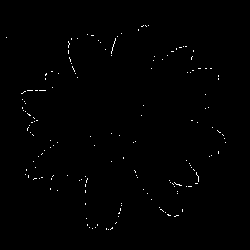
\includegraphics[width=0.99\textwidth]{images/Canny/flower_Matlabedge_Roberts.png}
    \captionof{figure}{Sobel}
\end{minipage}%
\begin{minipage}{.33\textwidth}
  \centering
  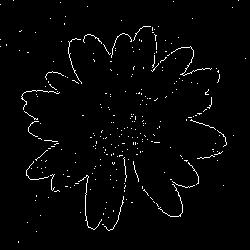
\includegraphics[width=0.99\textwidth]{images/Canny/flower_Matlabedge_Prewitt.png}
  \captionof{figure}{Prewitt}
\end{minipage}%
\begin{minipage}{.33\textwidth}
  \centering
  \includegraphics[width=0.99\textwidth]{images/Canny/flower_Matlabedge_Roberts.png}
  \captionof{figure}{Roberts}
\end{minipage}
\begin{minipage}{.33\textwidth}
  \centering
    \includegraphics[width=0.99\textwidth]{images/Canny/flower_Matlabedge_Canny_1.2.png}
    \captionof{figure}{Canny}
\end{minipage}%
\begin{minipage}{.33\textwidth}
  \centering
    \includegraphics[width=0.99\textwidth]{images/Canny/flowerFinal.png}
    \captionof{figure}{Nossa}
\end{minipage}%
\end{figure}



\end{document}
